\chapter{Sparse coding}
\label{chap:sparse_coding}
%Back to our initial problem of\ref{sec:dicts} $x = D\alpha$

The Cambridge Advanced Learner defines a code as
\begin{quotation}
``... a system of numbers, letters or signals which is used to represent
something in a shorter or more convenient form.''
\end{quotation}
A \emph{sparse code} is a vector with only a few non-zero coefficients
which is used to represent another vector by linear combine only few atom
vectors from a dictionary of many of them.

The idea of sparse coding of image signals has its origin in neural science. 
Research in this field found that the cells in the visual cortex, also known as
\emph{V1}, have properties similar to those localized filtering of wavelets
functions. Several approaches were made to create systems that resemble this
phenomena but did not lead to the desired structures. In 1996 Olshausen and
Field\cite{Olshausen1996} noticed that when adding a sparsity constraint to
these learning algorithms they can regenerate those characteristic elements.
%Following this discovery constraints were added to the least-squares problem.

\newpage % aragraph{}
Consider $\mat{X} \in \mathbb{R}^{m\times n}$  as a matrix with $n$ columns each
column $i$ representing a signal described by a single vector $\vec{x}_{i}$ of
signal length $m$. The dictionary $\mat{D}\in\mathbb{R}^{m \times p}$ is another
matrix with $p$ columns where each column $j$ represents an atom signal
$\vec{d}_j$ with the same dimension $m$ as a single signal $\vec{x}_{i}$ from
$\mat{X}$. The number of atoms $p$ in the dictionary is higher then the
dimension $m$ of the signals $p > m$ making the dictionary over-complete. The
sparse vector $\vec{\alpha}$ consists of coefficients $\alpha_i$ that can
describe a linear
combination of only a few non-orthogonal atoms from $\mat{D}$ that is close to
the signal $\vec{x}_i $ in $\mat{X}$. 

%Sparse coding is the 
\begin{align*}
\vec{x}_i = \underbrace{\begin{pmatrix} x_1 \\ x_2 \\ \vdots \\ x_n
\end{pmatrix}}_{signal}
\approx \underbrace{\begin{pmatrix} \vec{d}_1  \vec{d}_2 \cdots \vec{d}_n
\end{pmatrix}}_{\textrm{dictionary atoms}}
\underbrace{\begin{pmatrix} \alpha_1 \\ 0 \\ \vdots \\ \alpha_n
\end{pmatrix}}_{\textrm{sparse vector }}
\end{align*}

When signal $\vec{x}$ and dictionary $\mat{D}$ are known 
and $\vec{\alpha}$ is unkown the solution to this problem is a solve of an
under-determined linear system.
\begin{equation*}
 \vec{\alpha} = \mat{D}^{-1}\vec{x} 
\end{equation*}
The problem is not well-posed because there is more than one
solution to it. %Such a problem is called a ill-posed problem.
But we only need one of them. We want to find the sparsest
solution making the problem well-posed. To archive this it is necessary to keep
the coefficient vector $\vec{\alpha}$ sparse. 

\begin{figure}[h]
\centering
%\subfloat[over-complete]{\includegraphics[width =
%0.20\textwidth]{images/sparse_2.pdf}}
\hspace{5mm}
\subfloat[over-complete and sparse]{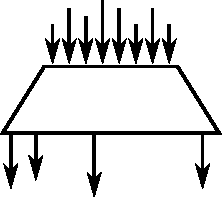
\includegraphics[width =
0.20\textwidth]{images/sparse.pdf}}
\caption{over-complete and sparse}
\label{fig:sparse}
\end{figure}

%\begin{figure}[h]
%\centering
%%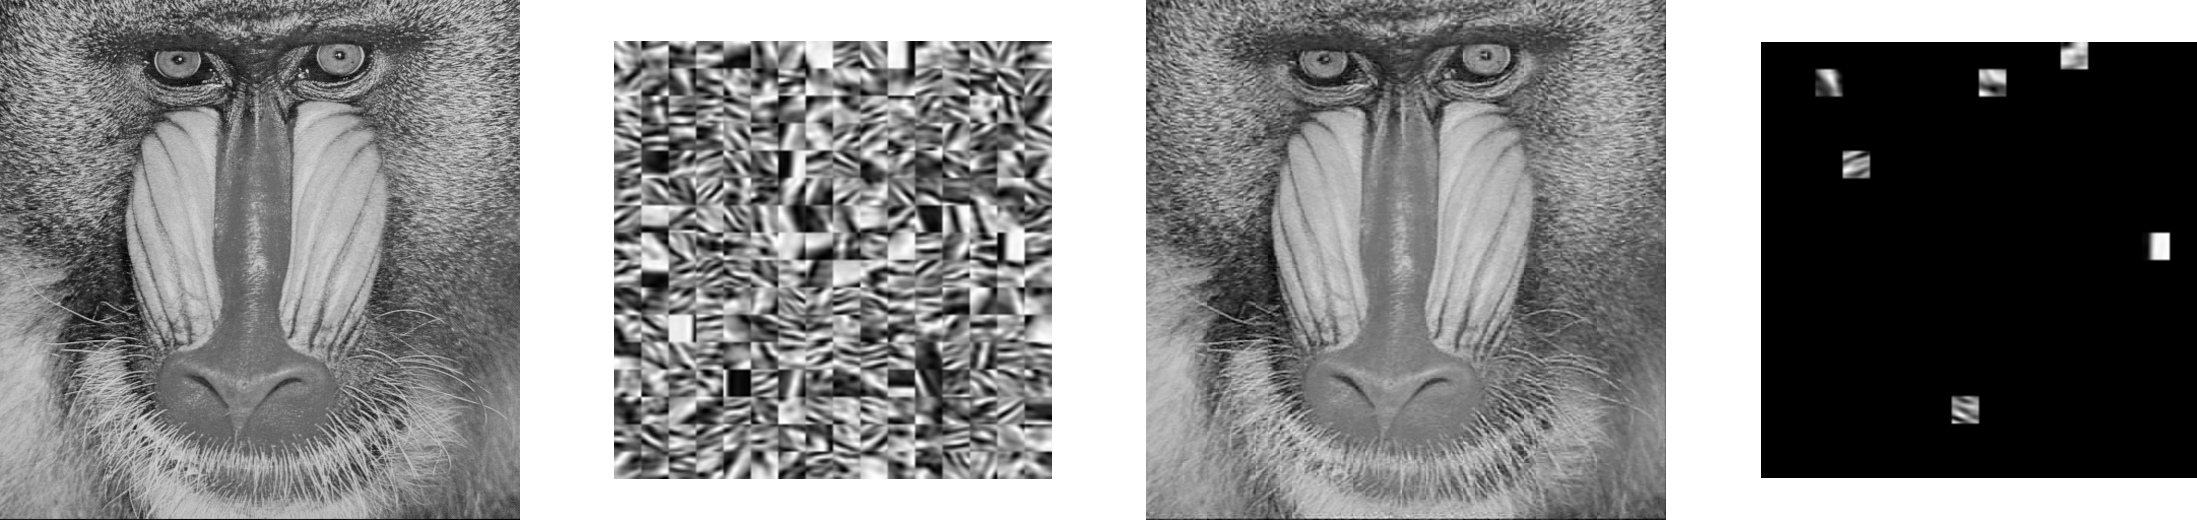
\includegraphics[width = 1.0\textwidth]{images/sparse_selection.pdf}
%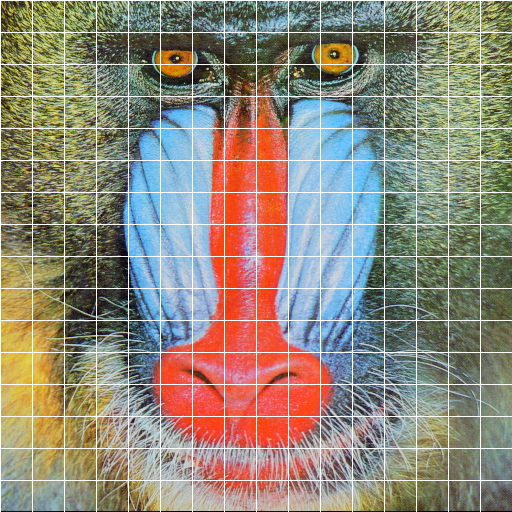
\includegraphics[scale = 0.25]{images/segmentation.png}
%\caption{}
%\label{fig:sparse}
%\end{figure}



\section{Regularization}
A regularization adds additional information to a problem in order to solve an
ill-posed problem or to prevent over-fitting.\footnote{\url{
http://en.wikipedia.org/wiki/Regularization_(mathematics)}}
To find the sparsest solution the sparse coding approach adds such
regularization to the the problem \ref{eq:problem}. 
%.. over-fitting .. Such a constraint is the regularization.
\begin{equation}
\min_{\vec{\alpha}\in\mathbb{R}^{p}}
\underbrace{\lVert \vec{x} -
\mat{D}\vec{\alpha}\rVert^{2}_{2}}_{error} \text{ s.t. }
\underbrace{\psi(\vec{\alpha})}_{regularization}\leq L \label{eq:problem}
%\min_{\vec{\alpha}\in\mathbb{R}^{p}} \lVert \vec{x} - \mat{D}\vec{\alpha}
%\rVert^{2}_{2}
\end{equation}
The regularization acts as a constraint to the structure of $\vec{\alpha}$. It
should be choosen in a way which keeps the number of non-zero coefficient of
$\vec{\alpha}$ low. 
This sparsity constraint can be achieved with the help of
the $\ell_0$-norm. The $\ell_0$-norm is a pseudo-norm that virtually counts the
number of non-zero elements in the vector in the form of:
\begin{equation*}
\lVert \vec{x} \rVert_{0} = \#\{i:\vec{x}[i] \neq 
0; i=1,...,n; \vec{x}\in\mathbb{R}^n\} 
\end{equation*}
There is one significant problem in using $\ell_0$-norm. This particular
regularization makes the initial problem \ref{eq:problem} NP-hard. To get the
ideal solution it is necessary to test every combination of atoms. But this
does not imply that there is no way to efficiently find a solution that is good
enough to keep $\alpha$ sparse. There exist several greedy algorithms that can
solve the problem in a not perfect but good enough way. 

Another regularization that can keep $\vec{\alpha}$ sparse is the use of the
$\ell_p$-norm.
\begin{equation*}
\lVert \vec{x}\rVert_p = \sum_{i=1}^n\left(\lVert \vec{x}[i]
\lVert^p\right)^{1/p}
\end{equation*}
With either the $\ell_1$-norm ($p=1$) or $\ell_2$-norm ($p=2$) as a
convex relaxation of the $\ell_0$-norm. Even though that the $\ell_1$-norm is
not the same as the $\ell_0$ it can be demonstrated that the $\ell_1$-norm is
equivalent to the $\ell_0$-norm in the effect of inducing sparsity. 
Figure \ref{fig:sparse} shows an example of regularization with two coefficients
of $\vec{\alpha}$ and the $\ell_p$-norm with $p=1$ and $p=2$.
%\Todo{image/description of different regularizations}
\begin{figure}[h]
\centering
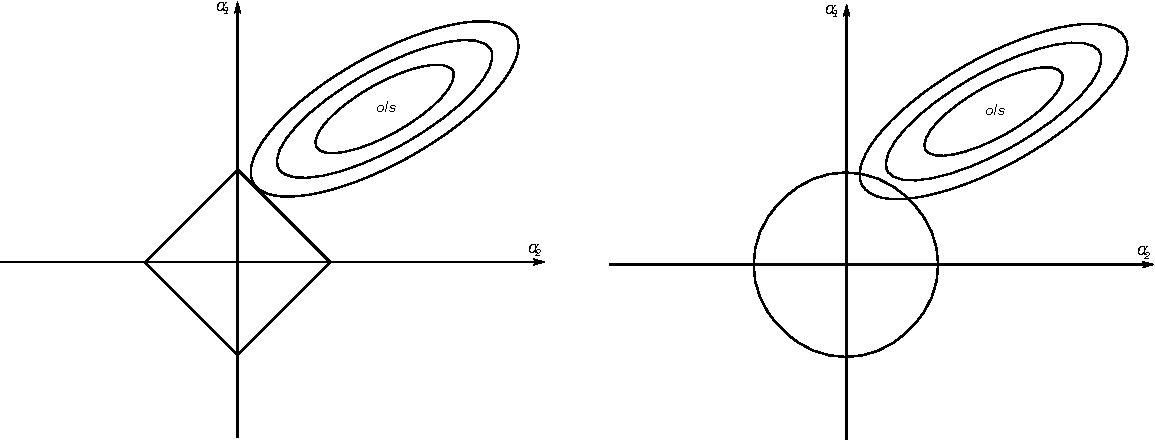
\includegraphics[width = 1.0\textwidth]{images/regularization.pdf}
\caption[$\ell_p$ regularization]{different $\ell_p$-norm hitting least-squares
solution}
\label{fig:sparse}
\end{figure}
When $\alpha_1$ of the ordinary least-squares(ols) solution hits zero the
$\ell_1$-norm will find a sparse solution while a $\ell_p$-norm with $p>1$ does
not necessarily procude sparsity.

In the past 15 years several sparse coding algorithms have been proposed. Some
that solve the initial $\ell_0$ regularized problem greedily, like
the (orthogonal)-matching-pursuit or FOCUSS and others which modified the
problem to become convex. The algorithms solve the convex problem  primary
derived from the numerical domain in the form of large linear system solvers
with few optimization constraints. The most common of them are the
Basis-pursuit, LARS-Lasso and Ridge regression. The next two sections give a
more in depth look on those algorithms. 

%$\ell_2$ Method Of Frames


%copy
% Following Tao et al., where it was shown that the L1 norm is equivalent to the
%L0 norm, 
%leads one to solve an easier problem. Finding the candidate with the smallest
%L1 norm can be expressed relatively
%easily as a linear program, for which efficient solution methods already exist.
%These solution methods have been refined over the past few years yielding
% enormous gain
%\begin{figure}
%\centering
%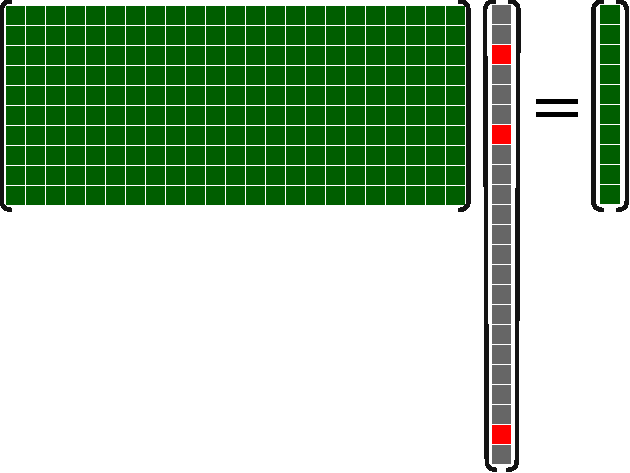
\includegraphics[width = 0.66\textwidth]{images/Da_x.pdf} % Or .pdf
%\caption{Sparse Coding}
%\label{fig:da_x}
%\end{figure}

\section{$\ell_0$ regularization with greedy algorithms}
%present a selection of the most common algorithms to solve the initial problem
%under a $\ell_0$ regularization.
We now have a more in depth look at two very popular algorithms. 
The matching-pursuit and its successor the orthogonal-matching-pursuit.
Both use a greedy strategy to calculate the coefficient vector $\vec{\alpha}$ to
find
a solution to the following NP-hard problem. By solving for
\begin{equation*}
\min_{\vec{\alpha}\in\mathbb{R}^{p}}   \lVert \vec{\alpha} \rVert_{0}   \textrm{
s.t. }
\lVert \vec{x} - \mat{D}\vec{\alpha} \rVert^{2}_{2} \leq \epsilon
\end{equation*}
respectively
\begin{equation*}
\min_{\vec{\alpha}\in\mathbb{R}^{p}}  \lVert \vec{x} - \mat{D}\vec{\alpha}
\rVert^{2}_{2} \textrm{ s.t.
} \lVert \vec{\alpha}	1 \rVert_{0} \leq L
\end{equation*}.

\subsection{Matching-Pursuit}
\label{sec:mp}
The matching-pursuit was first presented in 1993 by Mallat and
Zhang\cite{Mallat1993} on audio samples and later adapted to images by Mallat
and Bergeaud in\cite{Mallat1995}.
The algorithm starts with the coefficient vector $\alpha$ set
to zero. Then finds the atom in the dictionary with the best reduction of the
error. This is done by selecting the coefficient that has the maximum
correlation with the current remaining error (residual). This step is repeated
$L$ times or until the error $\epsilon$
% $\lVert \vec{x} - \mat{D}\vec{\alpha} \rVert^{2}_{2}$ 
for the current $\vec{\alpha}$ fullfills $\lVert \vec{x} - \mat{D}\vec{\alpha}
\rVert^{2}_{2} = \lVert \vec{r} \rVert_2^2 \leq \epsilon$.
%respectively the residual fulfills $\lVert \vec{r} \rVert_2 \leq \epsilon$.
Algorithm \prettyref{alg:mp} illustrates this procedure.
\begin{algorithm}[H]
\caption{Matching-Pursuit}
\label{alg:mp}
\begin{algorithmic}[1]
\REQUIRE $\vec{x} \in \mathbb{R}^m, \mat{D} \in \mathbb{R}^{m\times p}, L \in
\mathbb{N}, \epsilon \in \mathbb{R}$
\STATE $\vec{\alpha} \gets 0$ (start with zero vector)
\STATE $\vec{r} \gets \vec{x}-\mat{D}\vec{\alpha} = \vec{x}$ (residual) 
\WHILE {$\lVert \vec{\alpha} \rVert_{0} \leq L$ \AND $\lVert \vec{r} \rVert_2^2
\leq \epsilon$}
\STATE Select atom with maximum correlation with residual: 
\begin{equation*}
i \gets \argmax_{i=1,...,p} \lvert \left<\vec{d}_i,\vec{r}\right> \rvert
\end{equation*}
\STATE update coefficients: 
\begin{align}
\vec{\alpha[i]}  \gets \vec{\alpha[i]} + \left<\vec{d_i},\vec{r}\right>
\label{eq:mp_update}
\end{align}
\STATE update residual:
\begin{equation*}
 \vec{r} \gets \vec{r} - \left<\vec{d_i},\vec{r}\right>\vec{d_i}
\end{equation*}
\ENDWHILE
\RETURN $\vec{\alpha}$
\end{algorithmic}
\end{algorithm}

\subsection{Orthogonal-Matching-Pursuit}
\label{sec:omp}
The Orthogonal-Matching-Pursuit, an improved version of
the Matching-Pursuit (\ref{sec:mp}), was first presented by Pati et al.
in 1993\cite{Pati1993}. Rather than just updating the currently selected
coefficient of $\vec{\alpha}$ (\ref{eq:mp_update}). The algorithm re-evaluates
all coefficients in the current set $A$ of active atoms $\vec{\alpha}_A$ by
solving a full least-squares solution in every iteration (\ref{eq:omp_update}).
This improves the quality of the solution\cite{Pati1993}. The
Orthogonal-Matching-Pursuit gets its name from the fact that the residual
$\vec{r}$ is orthogonal to the previously selected atoms in dictionary
$\mat{D}$. This orthogonality property leads to the effect that every
coefficient is only selected once. Algorithm \ref{alg:omp} shows a
description in pseudocode.

\begin{algorithm}[H]
\caption{Orthogonal Matching Pursuit}
\label{alg:omp}
\begin{algorithmic}[1]
\REQUIRE $\vec{x} \in \mathbb{R}^m, \mat{D} \in \mathbb{R}^{m\times p}, L \in
\mathbb{N}, \epsilon \in \mathbb{R}$
\STATE $\vec{\alpha} \gets 0, \vec{r} \gets \vec{x} $ (residual) $, A \gets
\emptyset$
\FOR {$j = 0$ to $L$}
\STATE Select inactive variable with maximum correlation with residual: 
\begin{equation*}
i \gets \argmax_{i \in A^C} \lvert \left<\vec{d_i},\vec{r}\right> \rvert
\end{equation*}
\STATE update active set:
\begin{equation*}
 A \gets A \cup \{i\} 
\end{equation*}
\STATE update coefficients: 
\begin{align}
\vec{\alpha}_A \gets \left( \mat{D}_A^T \mat{D}_A \right)^{-1} \mat{D}_A^T x 
\label{eq:omp_update}
\end{align}\label{alg:OMP_DTD}
\STATE update residual: $\vec{r} \gets \vec{x}-\mat{D}_A\vec{\alpha}_A$
\ENDFOR
\RETURN $\vec{\alpha}$
\end{algorithmic}
\end{algorithm}
%Section \ref{sec:batch-omp} provides a depper look into the Batch-OMP.

All these greedy approaches tend to find suitable solutions but
because of the non-convex problem they can get stuck in a local minimum. As
shown before an $\ell_1$ regularization version of \ref{eq:problem} also keeps
the coefficient vector $\vec{\alpha}$ sparse but eliminates the problem of a
local minimum. The next section presents algorithms which solve  a $\ell_1$
regularization version of \ref{eq:problem}.


\section { $\ell_1$ regularization with the Lasso}
The $\ell_1$ regularization of our initial problem is also known as the
\emph{Lasso}. The name stands for \emph{least absolute shrinkage and
selection operator} and is a regularized version of a least-squares
solution. The sparsity is achieved by adding a constraint that induces
the $\ell_1$-norm of $\vec{\alpha}$ to be small. It was first
presented by
Tibshirani
in 1996\cite{Tibshirani1996}. Under this constraint our initial problem becomes:
\begin{equation}
\min_{\vec{\alpha}\in\mathbb{R}^{p}} \lVert \vec{x} - \vec{D}\vec{\alpha}
\rVert^{2}_{2} \textrm{
s.t. } \lVert \vec{\alpha} \rVert_{1} \leq L \label{eq:l1}
\end{equation}
Algorithms dealing with this problem often require to formulate the
constrained function into a single expression. The lagrange multiplier is a
method to construct such an expression from a function and a constraint. With
the  lagrange multiplier applied the regularized problem \ref{eq:l1} becomes:
\begin{equation}
\min_{\vec{\alpha}\in\mathbb{R}^{p}}  \frac{1}{2} \lVert \vec{x} -
\vec{D}\vec{\alpha} \rVert^{2}_{2} +
\lambda \lVert \vec{\alpha} \rVert_{1}\label{eq:l1lagrange}
\end{equation}
Where the coefficient $\lambda$ controls the sparsity in equivalent to $L$.
In the last two decades several algorithms were proposed to compute the
Lasso. The basis pursuit by Chen et al.\cite{Chen1995}, the FOCUSS\cite{FOCUSS}
, the LARS by Efron et al.\cite{Efron2004} among others. We have a more in-depth
look at the LARS-Lasso.


\subsection{LARS-Lasso}
\label{sec:lars}
% \Todo{split into LAR and LARS-lasso, better illustrate than use complex
%formulas}
The LARS-Lasso is an algorithm to solve the Lasso with the help of a regression
algorithm known as \emph{least-angle regression (LAR)}. Regression tries to find
the correlation between a depended variable, here \prettyref{eq:l1lagrange}, and
a set of independent variables, our coefficients of $\alpha$.
The LAR and LARS-Lasso were first presented in 2004 by Efron et
al.\cite{Efron2004}.


\paragraph{Least-angle regression}
The main idea of the least angle regression is to start with all coefficients
of $\vec{\alpha}$ set to zero and the residual gets $\vec{r}=\vec{x}$. Then
find the atom $\vec{d}_i$ of $\mat{D}$ with the maximum correlation
with the residual $\argmax_i\mat{d}_i\vec{r}$ and move $\alpha_i$ 
into the direction of the least-squares solution until a new atom
$\vec{d}_j$ has the same or higher correlation with the residual. Now move
$\vec{\alpha}[i]$ and $\vec{\alpha}[j]$ into the joint direction of the
least-squares
solution until another atom has the same or higher correlation with $\vec{r}$.
Repeat this procedure until the desired number of atoms are selected.

%The complete regularization path based on\cite{Efron2004}
%\begin{align}
%\min_{\vec{\alpha}\in\mathbb{R}^{p}}  \frac{1}{2} \lVert \vec{x} -
%\vec{D}\vec{\alpha} \rVert^{2}_{2} + \lambda \lVert \vec{\alpha} \rVert_{1}
%\end{align}


\paragraph{Lasso modification}
The LAR algorithm can be easily modified to solve the Lasso. 
The modification consists of removing an atom $\vec{d}_i$ from the active set
when their coefficient $\alpha_i$ becomes zero. A pseudocode implementation can
be found in \prettyref{alg:lars}.

\paragraph{}
We have to admit that the LARS-Lasso algorithm has some limitations concerning:
\begin{description}
 \item[Dimension] When the dimension $m$ of a signal $\vec{x}$ is much
higher than the number of atoms $p$ of the dictionary $\mat{D}$ the algorithm
can only select $p$ columns.
  \item[Correlation] When the columns of the dictionary are highly correlated
the algorithm selects only one column.
\end{description}
The first limitation is not relevant for our experiments as our dictionaries
are over-complete, with respect to the dimension $m$ of signal $\vec{x}$, and
thus satisfy $m \leq p$. 



\begin{algorithm}[H]
\caption{LARS-Lasso}
\label{alg:lars}
\begin{algorithmic}[1]
\REQUIRE $\vec{x} \in \mathbb{R}^m, \mat{D} =[\vec{d}_1,...,\vec{d}_p] \in
\mathbb{R}^{m\times p} \text{normalized and centered},\lambda \in \mathbb{R}$
\STATE $\vec{\alpha}_0 \gets 0, \vec{r}_0 \gets \vec{x}, A \gets \emptyset, n
\gets 0$

\WHILE {$\lVert\vec{\alpha}_n\rVert_2 < \lambda$}
\STATE calculate correlations with residual: $\vec{c} \gets
\mat{D}^T\vec{r}_n$
\STATE Select atom with maximum correlation: 
\begin{equation*}
i \gets \argmax_{i \in A^C} \lvert c_i  \rvert % \left<d_i,x-\mu_{j}\right>
\end{equation*}
\STATE maximum correlation: $c_{max} \gets c_i $ %\left<d_a,r\right> $
\STATE update active set: $A \gets A \cup \left\{i\right\} $
\STATE\COMMENT {calculate movement into least-squares direction}
\STATE signs of the correlations: $\vec{s} \gets  sign\left(\vec{c}_A\right)$
\STATE $\tilde{\mat{D}_A} \gets \mat{D}_A\left(\ldots s_i\vec{d}_i
\ldots\right)_{i\in A}$
\STATE $\mat{G}_A \gets \tilde{\mat{D}_A}^T\tilde{\mat{D}_A}$
\STATE calculate angle: $\beta \gets \sqrt{ \vec{1}_A^{-1} \mat{G}_A^{-1}
\vec{1}_A
}$
\STATE calculate weights: $\vec{w} \gets \beta\mat{G}_A^{-1}\vec{1}_A$
\STATE equiangular direction: $\vec{u} \gets \mat{D}_A\vec{w}$
%\STATE correlation between direction and variables: $\vec{a} \gets
%\mat{D}_t\vec{u}_A$
\STATE calculate movement:
\begin{equation*}
%\gamma \gets \min_{i\in A^C}^{+} \left\lbrace \frac{c_{max}-c_i }{A_A-a_i },
%\frac{c_{max}+c_i }{A_A+a_i } \right\rbrace
\gamma \gets \min_{j\in A^C}^{+} \left\lbrace \frac{c_{max}-\left<
\vec{x},\vec{d}_j \right> }{1-\left< \vec{d}_i,\vec{d}_j \right> },
\frac{c_{max}+\left< \vec{x},\vec{d}_j \right>}{1+\left< \vec{d}_i,\vec{d}_j
\right> } \right\rbrace
\end{equation*}

\IF {\COMMENT {Lasso modification}} 
%drop coefficient from active set that change sign
\STATE $ \tilde{\gamma} \gets -\vec{\alpha}_n/\vec{s}^T\vec{w}  $
\STATE $ i \gets \min_{i\in A}^{+} \left( \tilde{\gamma}_i \right) $
%\STATE $ i \gets \alpha_{i} = 0, i \in A $
\IF {$\tilde{\gamma}_i>0$ \AND $\tilde{\gamma}_i<\gamma$}
\STATE remove $i$ from active  set: $ A \gets A \backslash \{i\} $
\STATE update movement: $ \gamma \gets \tilde{\gamma}_i $  
\ENDIF
\ENDIF
%\STATE $ \mu_{j+1} \gets \mu_{j} - \gamma x_i $
\STATE update residual: $ \vec{r}_{n+1} \gets \vec{r}_{n} - \gamma \vec{u}
$
\STATE update coefficients: $ \vec{\alpha}_{n+1} \gets \vec{\alpha}_n - \gamma
\vec{s}^T\vec{w} $
\STATE $n \gets n + 1$ 
\ENDWHILE
\RETURN $\vec{\alpha}$
\end{algorithmic}
\end{algorithm}



\section{Application and Related Work}
In the most applications and papers related to sparse coding, the coding
step and the dictionary learning step are often close tied together. This
section concentrates on work with the main focus on sparse coding. Section
\ref{sec:related_dictionarie} shows related work where the learning of
dictionaries is the dominating part.

%\begin{description}
\paragraph{Noise reduction}
Is the process of remove noise $\vec{w}$ from a signal $\vec{y}$ gaining the
de-noised signal $\vec{x}$.
\begin{align*}
\vec{y} = \vec{x} + \vec{w}
\end{align*}
Using the fact that sparse coding is an approximation of signal that loses ...
noise? ... in its encoding process. 
Elad and Aharon showed in 2006\cite{Elad2006}.

\paragraph{In-painting}
Fill missing parts by removing rows from the dictionary.
Train with the original image
\begin{align*}
\vec{x} \approx \mat{D}\vec{\alpha}\\
\vec{x}_S \approx \mat{D}_S\vec{\alpha}\\
Wx \approx WD\alpha\text{select subset}\\
\end{align*}
Examples for this can be found in\cite{mairal08sparse}.

%Task driven dictionaries

\paragraph{Inverse half-toning} Half-toning, as used in printing, is a process
where a binary raster simulates continuous tone images. Small dots of different
size and shape create the optical illusion of continuous tones. In 2010 research
by Mairal et al.\cite{Mairal2010b} presented ...


\paragraph{Super resolution} \cite{Wright2008,Yang2010, Yang2010}  
Or the ongoing work by Couzinie-Devy et al., 2010 called digital zooming.


\paragraph{Structured sparsity}
similar patches should admit similar patterns \cite{Mairal2009} 
\cite{group sparsity}
\Todo{picture with distribution difference}

%\paragraph{Background subtraction}\cite{}
%\paragraph{Sense sparse signals}\cite{Duarte2009}







